The purpose of "Bluetooth Hydrometer" is to help users to digitally keep track of useful data such as temperature and specific gravity (SG) of beer during the fermentation process. Intended audiences, mostly home brewers, would be able to check temperature and SG constantly with the help of smartphone or computer..

\subsection{Purpose and Use}
Arduino nano 33 BLE is a Bluetooth enabled device that can receive analog and digital data from external sensors, temperature sensors in our case. Built in Gyroscope sensor would be able to help in determining SG of denser liquids such as beers which is ideal for Bluetooth Hydrometer. Sending temperature and SG data to smartphones or a website is another huge part of this project which involves building an app for smartphones and creating websites.
\subsection{Intended Audience}
Intended audiences are mostly brewers who love to ferment and create a variety of beers at home. Home brewers would be able to leave the device floating inside the fermentation vessel during the period of fermentation. Bluetooth Hydrometer is a standalone product which is not designed to be a part of a bigger system as of now. 

\begin{figure}[h!]
	\centering
   	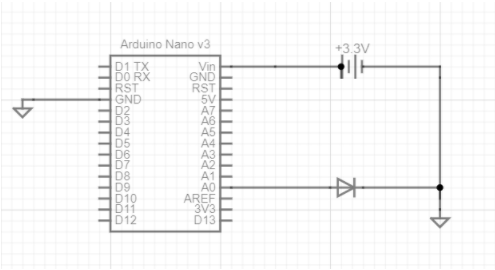
\includegraphics[width=0.60\textwidth]{images/arduino_nano_v3_schematic}
    \caption{Bluetooth Hydrometer}
\end{figure}
Conceptual Drawing